\chapter{Results}

	In this chapter the results of GPU design choices and algorithmic
	optimizations and their effects are reviewed.

	\section{Software Shader Performance}

		The shader performed as expected, a conventional graphics card is 
		capable of rendering scenes with low scene complexity in real-time
		using sphere tracing.

		However scenes can easily be made to look a lot more complex than they
		are, for example, by using mod fields,or modulo fields, when the modulo
		operation is used on an object it creates a field with multiple copies
		of the original object next to each other, or fractals. The hardware
		(Geforce GTX 1060M) that the shader was tested on was able to render 20
		reflective spheres in real time in fullHD using our performance
		enhancing algorithm.


	\section{GPU}
	
	The GPU has been tested by simulating it and running a program on it that 
	renders a sphere using Sphere Tracing. It spawns threads progressively to 
	fill the screen data buffer with pixels. The execution of our test programs 
	ran exactly as intended, with any number of simulated cores. The design has 
	also been put through a synthesizing tool for FPGAs, which creates a net 
	list of the components and connections that constitute the GPU. This also 
	works as intended without any unexpected problems, but the actual operation 
	of the GPU on an FPGA has not yet been verified.
	
	
	\section{Square roots}
		
		The accuracy of the different square root approximation and calculation
		methods are shown in figures \ref{sres1}, \ref{sres2}, \ref{sres3},
		\ref{sres4}, \ref{sres5}, and \ref{sres6}. The shifting nth root
		algorithm is used as a reference in all figures because it is always
		bit-accurate for integer square roots.

		\begin{figure}[H]
			\centering
			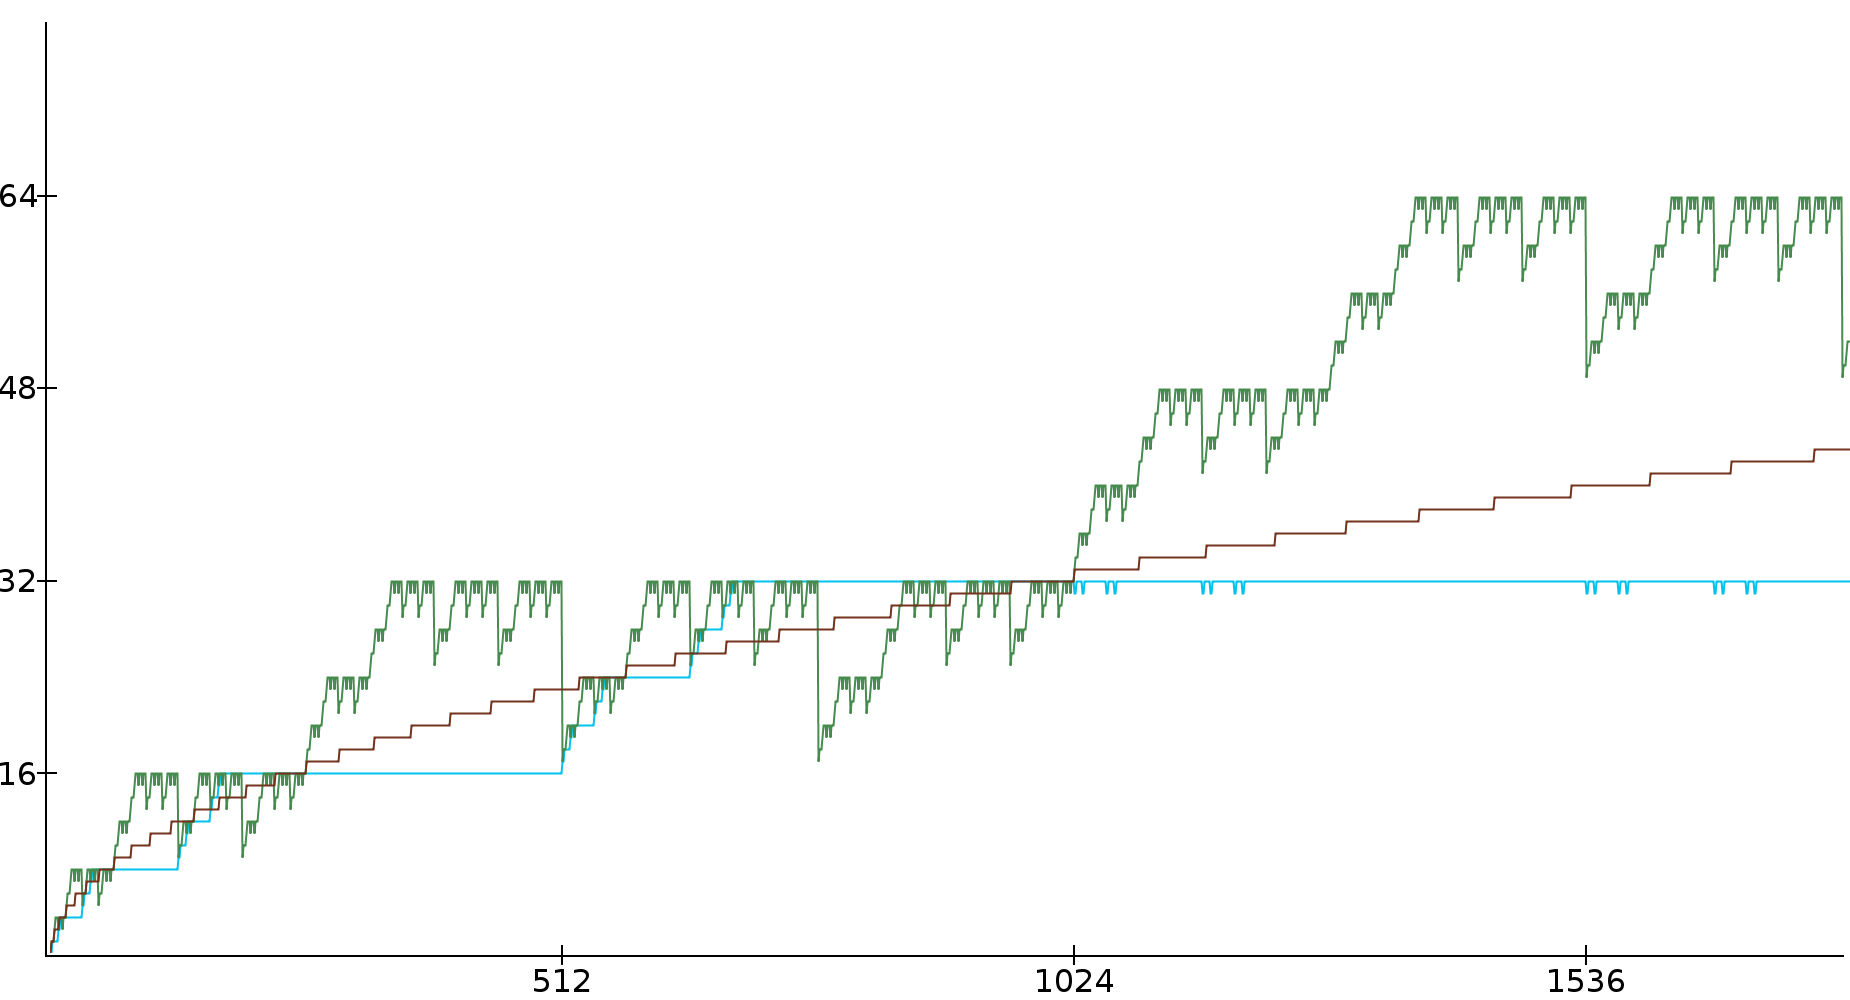
\includegraphics[width=0.75\linewidth]{figure/value12x.png} 
			\caption{Value from the simple square root approximator (green),
				the improved version (blue), and the shifting nth root 
				algorithm (red).}
			\label{sres1}
		\end{figure}

		\begin{figure}[H]
			\centering
			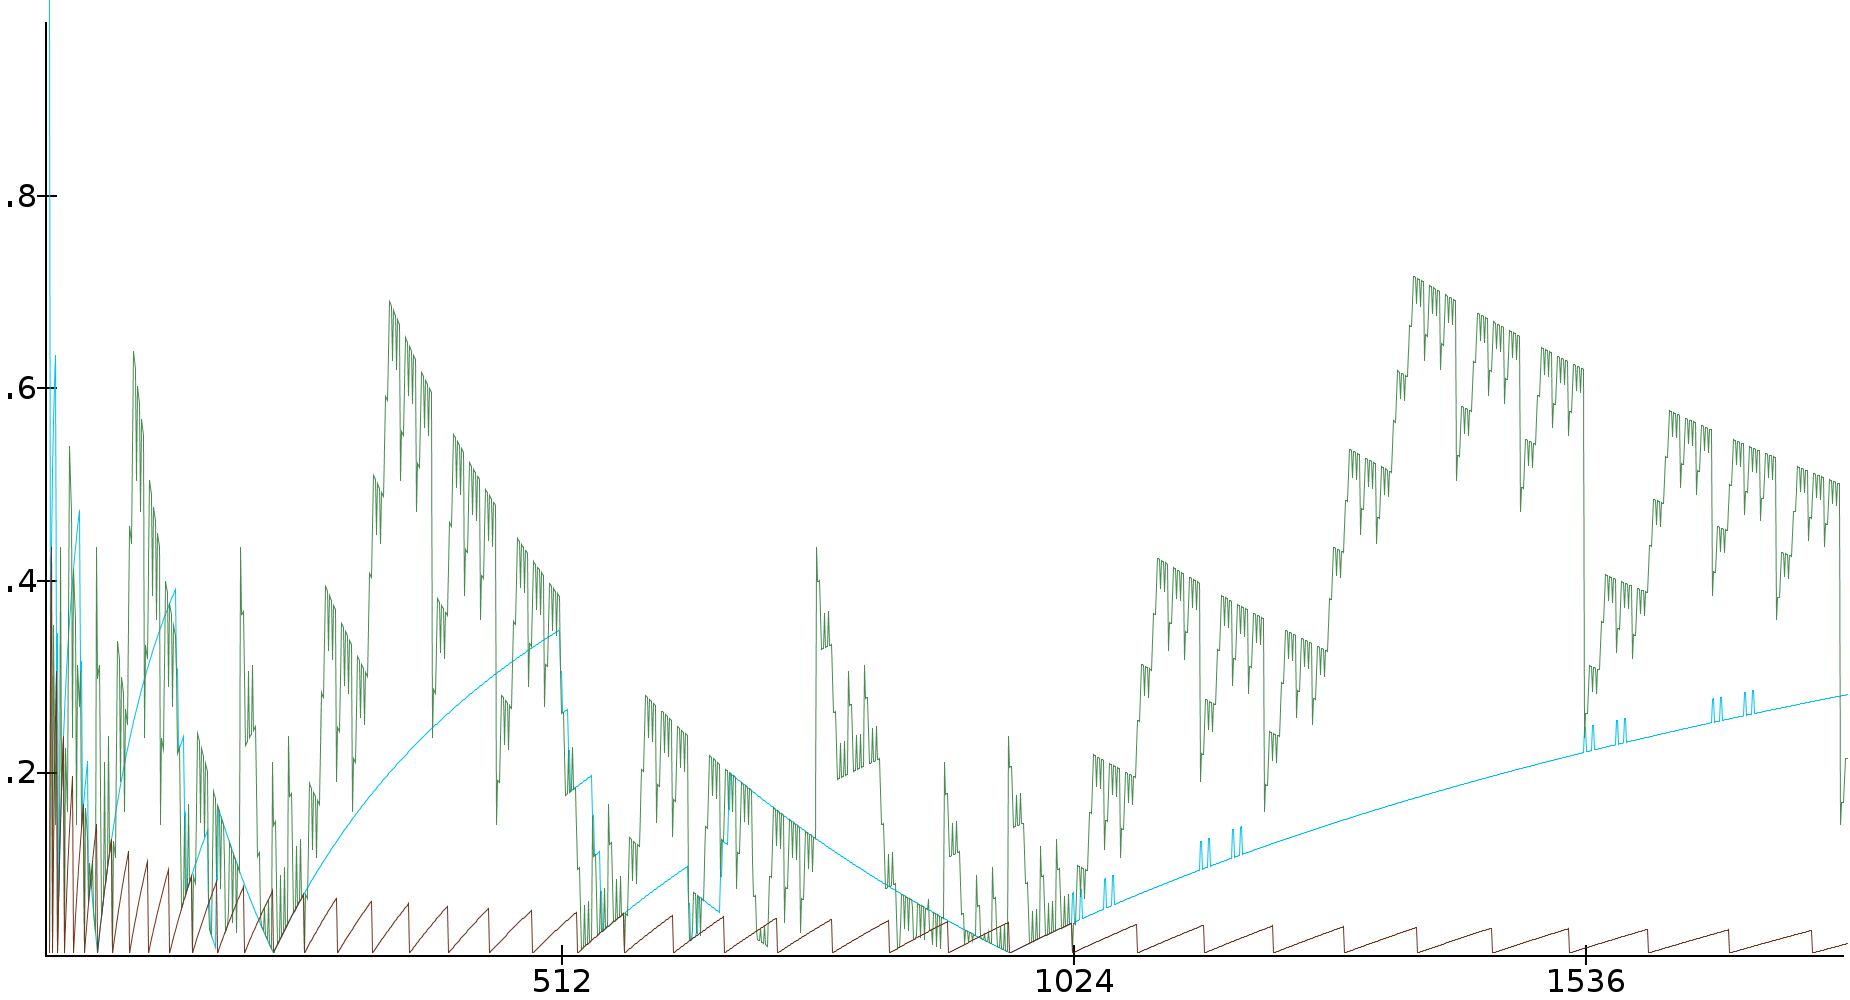
\includegraphics[width=0.75\linewidth]{figure/rel_error_480x.png} 
			\caption{Relative error for the simple square root approximator
				(green), the improved version (blue), and the shifting nth root
				algorithm (red).}
			\label{sres2}
		\end{figure}

		\begin{figure}[H]
			\centering
			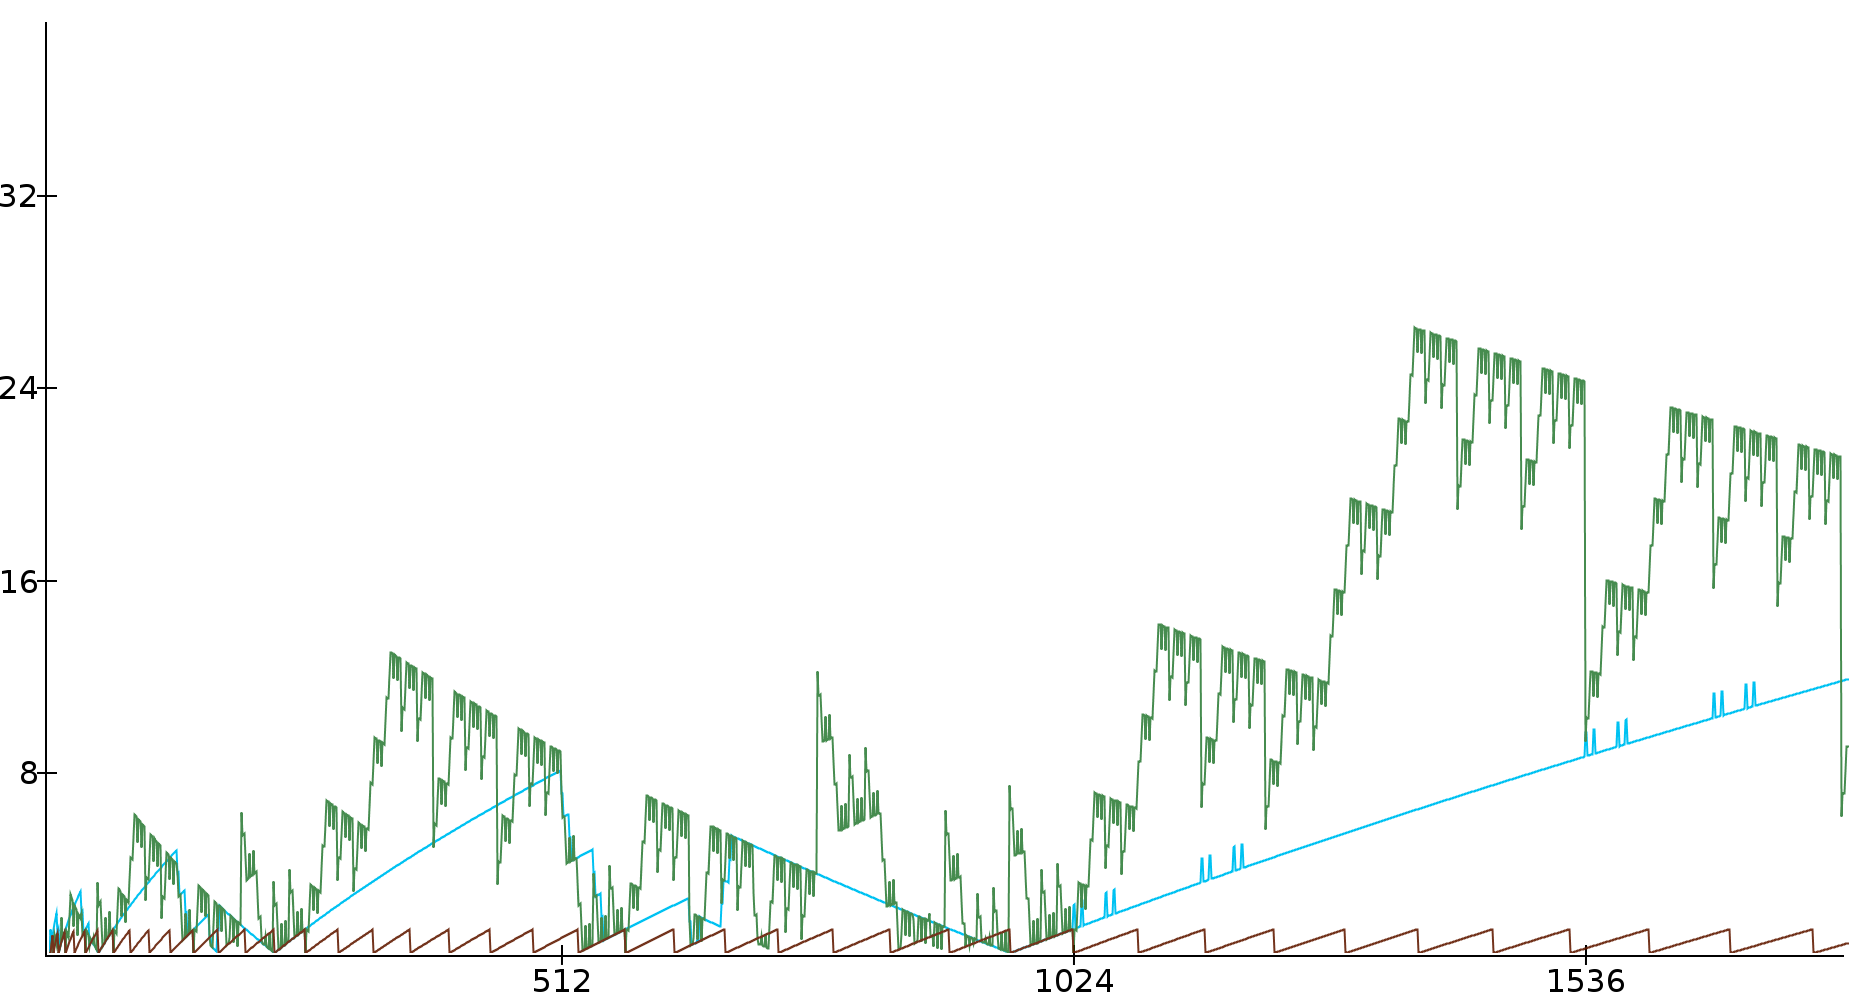
\includegraphics[width=0.75\linewidth]{figure/abs_error_24x.png} 
			\caption{Absolute error for the simple square root approximator
				(green), the improved version (blue), and the shifting nth root
				algorithm (red).}
			\label{sres3}
		\end{figure}

		\begin{figure}[H]
			\centering
			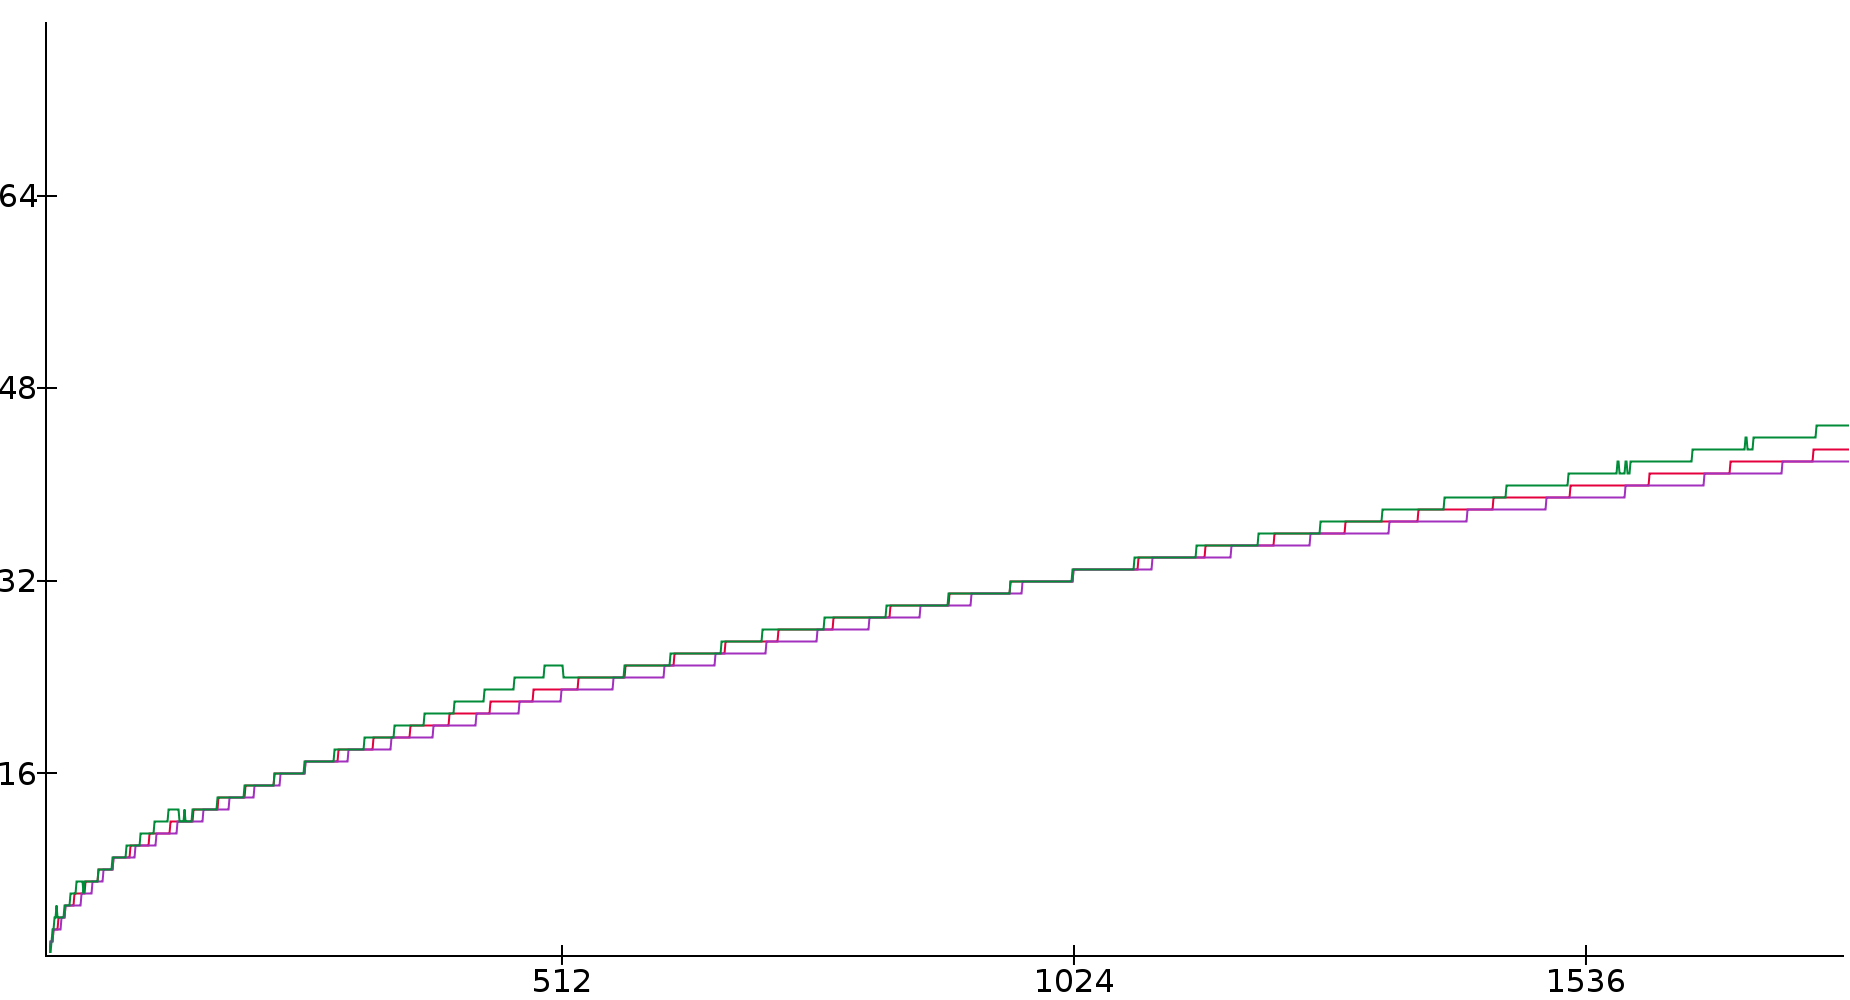
\includegraphics[width=0.75\linewidth]{figure/value_lin12x.png} 
			\caption{Value from lerp-approximator (purple), simple square root
				approximator with one step of the babylonian method (green),
				and the shifting nth root algorithm (red).}
			\label{sres4}
		\end{figure}

		\begin{figure}[H]
			\centering
			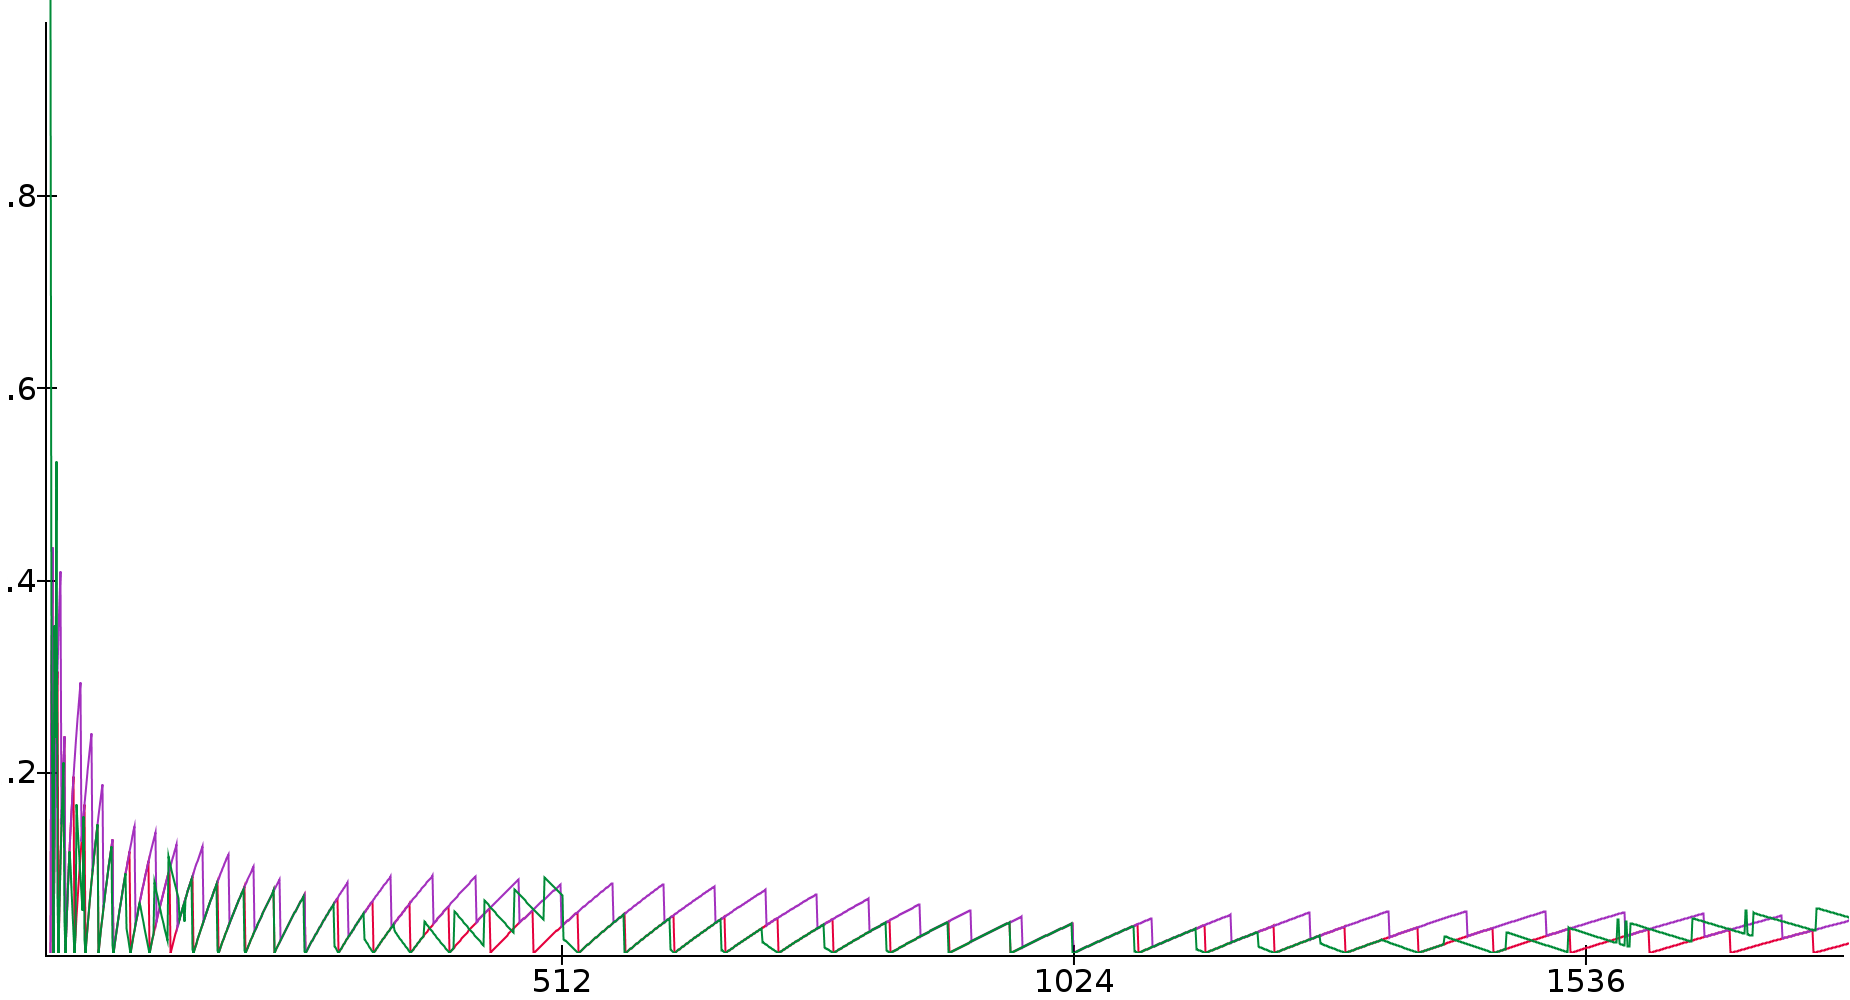
\includegraphics[width=0.75\linewidth]{figure/rel_lin960x.png} 
			\caption{Relative error for the lerp-approximator (purple), simple 
				square root approximator with one step of the babylonian method 
				(green), and the shifting nth root algorithm (red).}
			\label{sres5}
		\end{figure}

		\begin{figure}[H]
			\centering
			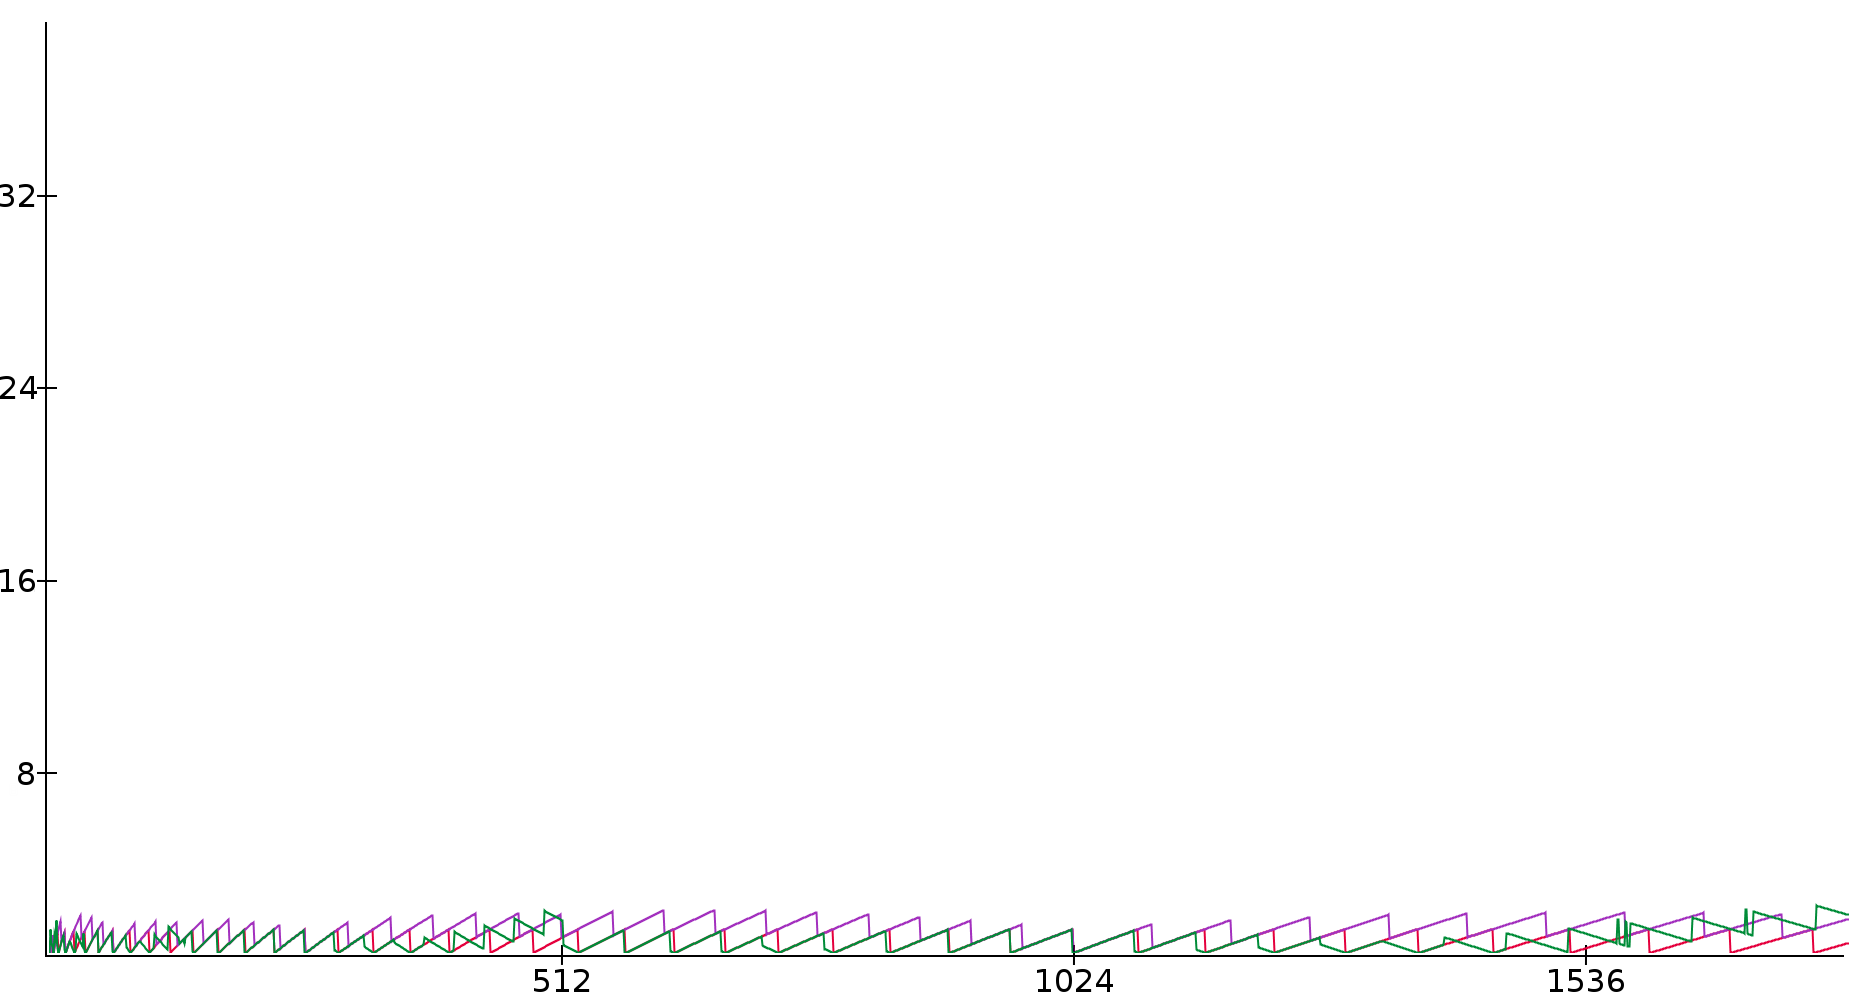
\includegraphics[width=0.75\linewidth]{figure/abs_lin24x.png} 
			\caption{Absolute error for the lerp-approximator (purple), simple 
				square root approximator with one step of the babylonian method 
				(green), and the shifting nth root algorithm (red).}
			\label{sres6}
		\end{figure}

	\section{Optimizations}
		
		During this project, a number of optimizations were discussed and
		developed. Implemented optimizations are explained below and the 
		theoretical ones are brought up in chapter \ref{discussion} and \ref{optimization}. 
		Some of these are based on earlier work, with some others believed 
		to be quite unique optimizations that have not been discussed for 
		sphere tracing previously. All implemented optimizations that affects
		the algorithm were implemented in the software shader, not on our own
		GPU.

		\subsection{Orthogonal culling}
		
		Tests to see the performance of the orthogonal culling optimization
		were performed by putting an increasing number of
		solid-colored spheres in a plane in front of the camera. Because of
		this, the spheres are not obstructed by other spheres, making this
		the best possible scenario for the optimization.

		Below are test results from Orthogonal culling.

			\begin{table}
			\centering
			\begin{tabular}{lll}
				\hline
				Objects & Optimized & Unoptimized \\ 
				\hline
				1       & 600       & 350         \\ 
				5       & 430       & 180         \\			
				10      & 290       & 98          \\
				15      & 85        & 13          \\
				20      & 58        & 9           \\
				25      & 40        & 6           \\
				30      & 29        & 4           \\
				35      & 7         & 3           \\
				40      & 6         & 2           \\
				45      & 4         & 1.5         \\
				\hline
			\end{tabular}
			\caption{Frames generated per second using the GLSL shader with and
				without the orthogonal culling optimization.}
			\end{table}

			%CHARTS
			
			\begin{table}
			\scatterplot{1,2,10,15,20,25}{50,100,150,200,250,300}{4}{0.33}{x}{y}{/figure/OptimizedGraf.txt}
			\end{table}



%  \scatterplot{x1,x2,x3...}{y1,y2,y3}{xscale}{yscale}{xlabel}{ylabel}{datafile}
%    where datafile is a file with a list of x y coordinates (one space 
%    separated pair on each line)






			The tests were performed by putting an increasing number of
			solid-colored spheres in a plane in front of the camera. Because of
			this, the spheres are not obstructed by other spheres, making this
			the best possible scenario for the optimization.

		\subsection{Bounding spheres}

			Bounding spheres were implemented and tested. There was a clear
			gain in performance in some cases, but the results are very situational, 
			depending on too many factors to be able to review (number of objects, 
			the dispersion of objects, size and place of the bounding sphere, etc.). 
			The larger the bounding sphere, the less performance gain will be seen 
			and the more objects that can fit into a bounding sphere the more performance 
			gain will be seen. 
